\chapter{Architecture technique}

% À charge à nous de remplir cette partie
% Indications :
%  Différents serveurs, postes de travail, réseaux...
% 
% Bon courage ;-)

\section{Architecture technique générale}
La solution est prévue pour fonctionner sur l'architecture générale présentée dans la figure \ref{ArchitectureGenerale}.
\begin{figure}[htbp]
	\centering
	\begin{tikzpicture}
		% Définition des styles
		\tikzstyle{sup} = [rectangle,draw=white,text=black,text centered,minimum width=20mm,minimum height=80mm]
		\tikzstyle{one} = [fill=colone,rectangle,draw=white,minimum width=20mm]
		\tikzstyle{two} = [fill=coltwo,rectangle,draw=white,minimum width=20mm]
		\tikzstyle{three} = [fill=colthree,rectangle,draw=white,minimum width=20mm]
		\tikzstyle{four} = [fill=colfour,rectangle,draw=white,minimum width=20mm]
		\tikzstyle{five} = [fill=colfive,rectangle,draw=white,minimum width=20mm]
		\tikzstyle{six} = [fill=colsix,rectangle,draw=white,minimum width=20mm]
		\tikzstyle{seven} = [fill=colseven,rectangle,draw=white,minimum width=20mm]
		\tikzstyle{inf} = [rectangle,draw=white,text=black,text centered,minimum width=20mm,minimum height=10mm]
		\tikzstyle{oneonthree} = [minimum height=26mm]
		\tikzstyle{twoonthree} = [minimum height=28mm]
		\tikzstyle{threeonthree} = [minimum height=26mm]
		\tikzstyle{oneonfour} = [minimum height=20mm]
		\tikzstyle{twoonfour} = [minimum height=20mm]
		\tikzstyle{threeonfour} = [minimum height=20mm]
		\tikzstyle{fouronfour} = [minimum height=20mm]
		\tikzstyle{arrow}=[->,>=latex,thick,rounded corners=4pt]
		% Noeuds utilisateurs
		\node[inf,one] at (  0mm, 0mm) {\centering\tiny\bfseries\scshape Utilisateurs};
		\node[one,oneonthree] (Utilisateurs) at (  0mm,18mm) {};
		\node at (  0mm,9mm) {\centering\tiny\itshape Métier};
		\node at (  0mm,19mm) {\centering\includegraphics[height=16mm]{"Logistician"}};
		\node[one,twoonthree] (Logistician) at (  0mm,45mm) {};
		\node at (  0mm,36mm) {\centering\tiny\itshape Logisticien};
		\node at (  0mm,46mm) {\centering\includegraphics[height=16mm]{"Logistician"}};
		\node[one,threeonthree] (Administrateur) at (  0mm,72mm) {};
		\node at (  0mm,63mm) {\centering\tiny\itshape Administrateur};
		\node at (  0mm,73mm) {\centering\includegraphics[height=16mm]{"Logistician"}};
		% Noeuds matériels
		\node[inf,two] at ( 20mm, 0mm) {\centering\tiny\bfseries\scshape Matériels};
		\node[two,oneonthree] (Matériels) at ( 20mm,18mm) {};
		\node at ( 20mm,9mm) {\centering\tiny\itshape Portable};
		\node at ( 20mm,19mm) {\centering\includegraphics[width=16mm]{"Laptop computer"}};
		\node[two,twoonthree] (Smartphone) at ( 20mm,45mm) {};
		\node at ( 20mm,36mm) {\centering\tiny\itshape Smartphone};
		\node at ( 20mm,46mm) {\centering\includegraphics[height=16mm]{"Smartphone"}};
		\node[two,threeonthree] (Satphone) at ( 20mm,72mm) {};
		\node at ( 20mm,63mm) {\centering\tiny\itshape Téléphone satellite};
		\node at ( 20mm,73mm) {\centering\includegraphics[height=16mm]{"Smartphone"}};
		% Noeuds application
		\node[inf,three] at ( 40mm, 0mm) {\centering\tiny\bfseries\scshape Application(s)};
		\node[three,minimum width=20mm,minimum height=80mm] (Application) at ( 40mm,45mm) {\centering};
		% Noeuds synchronisation
		\node[inf,four] at ( 60mm, 0mm) {\centering\tiny\bfseries\scshape Synchro};
		\node[four,oneonfour] (Physique1) at ( 60mm,15mm) {};
		\node at ( 60mm, 9mm) {\centering\tiny\itshape Physique};
		\node at ( 56mm,16mm) {\centering\includegraphics[width=6mm]{"Compact disk"}};
		\node at ( 64mm,16mm) {\centering\includegraphics[width=8mm]{"USB key"}};
		\node[four,twoonfour] (Internet1) at ( 60mm,35mm) {};
		\node at ( 60mm,29mm) {\centering\tiny\itshape Internet};
		\node at ( 60mm,36mm) {\centering\includegraphics[width=16mm]{"Internet"}};
		\node[four,threeonfour] (Téléphonie1) at ( 60mm,55mm) {};
		\node at ( 60mm,49mm) {\centering\tiny\itshape Téléphonie};
		\node at ( 60mm,56mm) {\centering\includegraphics[height=16mm]{"Phone antenna"}};
		\node[four,fouronfour] (Satellite1) at ( 60mm,75mm) {};
		\node at ( 60mm,69mm) {\centering\tiny\itshape Satellite};
		\node at ( 60mm,76mm) {\centering\includegraphics[height=16mm]{"Satellite"}};
		% Noeuds serveur local
		\node[inf,five] at ( 80mm, 0mm) {\centering\tiny\bfseries\scshape\begin{tabular}{c}Serveur \\ local\end{tabular}};
		\node[five,minimum height=80mm] (Server1) at (80mm,45mm) {};
		\node at (80mm,34mm) {\centering\tiny\itshape Serveur};
		\node at (80mm,48mm) {\centering\includegraphics[width=16mm]{"Server"}};
		% Noeuds synchronisation
		\node[inf,six] at (100mm, 0mm) {\centering\tiny\bfseries\scshape Synchro};
		\node[six,oneonfour] (Physique1) at (100mm,15mm) {};
		\node at (100mm, 9mm) {\centering\tiny\itshape Physique};
		\node at ( 96mm,16mm) {\centering\includegraphics[width=6mm]{"Compact disk"}};
		\node at (104mm,16mm) {\centering\includegraphics[width=8mm]{"USB key"}};
		\node[six,twoonfour] (Internet2) at (100mm,35mm) {};
		\node at (100mm,29mm) {\centering\tiny\itshape Internet};
		\node at (100mm,36mm) {\centering\includegraphics[width=16mm]{"Internet"}};
		\node[six,threeonfour] (Téléphonie2) at (100mm,55mm) {};
		\node at (100mm,49mm) {\centering\tiny\itshape Téléphonie};
		\node at (100mm,56mm) {\centering\includegraphics[height=16mm]{"Phone antenna"}};
		\node[six,fouronfour] (Satellite2) at (100mm,75mm) {};
		\node at (100mm,69mm) {\centering\tiny\itshape Satellite};
		\node at (100mm,76mm) {\centering\includegraphics[height=16mm]{"Satellite"}};
		% Noeuds serveur central
		\node[inf,seven] at (120mm, 0mm) {\centering\tiny\bfseries\scshape\begin{tabular}{c}Serveur \\ central\end{tabular}};
		\node[seven,minimum height=80mm] (Server2) at (120mm,45mm) {};
		\node at (120mm,34mm) {\centering\tiny\itshape Serveur};
		\node at (120mm,48mm) {\centering\includegraphics[width=16mm]{"Server"}};
		\end{tikzpicture}
	\caption{Architecture générale}
	\label{ArchitectureGenerale}
\end{figure}

\subsection{Matériels}
\mo possède déjà de nombreux matériels normalisés. La solution a donc été prévue pour fonctionner pleinement sur ces derniers~:
\begin{itemize}
	\item serveurs (locaux et central) actuellement sous Microsoft~Windows (une migration vers une distribution GNU/Linux étant en projet). Le stockage actuel des données est pris en charge par deux SGBDR que sont MySQL~Server et SQL~Oracle~;
	\item d'ordinateurs portables sous Microsoft~Windows~7. Ils sont équipés de 16 Go de mémoire vive et de 250 Go d'espace disque. \href{https://www.microsoft.com/fr-fr/download/internet-explorer.aspx}{Microsoft~Internet~Explorer~11} et \href{http://www.mozilla.org/en-US/firefox/27.0.1/releasenotes/}{Mozilla~Firefox~27.0.1} sont les deux navigateurs présents par défaut et leur utilisation est fonction des préférences de l'utilisateur~;
	\item de terminaux satellitaires \href{http://explorersatellite.com/BGAN/thrane_thrane_bgan.html}{BGAN (Thrane \& Thrane~Explorer~500)}~;
	\item de smartphones sous \href{http://www.android.com/}{Android}~;
	\item de téléphones satellitaires Thuraya (\href{http://www.thuraya.com.kw/hughes7101.html}{Hughes~7100} / \href{http://www.thuraya.com.kw/hughes7100.html}{7101} et \href{http://www.thuraya.com.kw/so-2510.html}{SO~2510}) et Iridium (\href{http://www.iridium.com/products/Iridium-9505A-Satellite-Phone.aspx}{9505A} et \href{http://www.iridium.com/products/Iridium9555SatellitePhone.aspx}{9555}) destinés principalement à la communication vocale~;
	\item de téléphones télécopieurs (fax) satellitaires (Nera~Mini-M~Worldphone)~;
	\item de communicateurs radio VHF (Motorola~GP360/GM360)~;
	\item de points d'accès sans fil (Linksys~WRT54G) permettant de partager une connexion à large bande (BGAN, ADSL, VSAT, etc.) dans un réseau sans fil.
	\item de GPS portables (eTrex~Venture~HC de Garmin).
\end{itemize}
\begin{constraint}[Contrainte de compatibilité]
La suite logicielle doit impérativement être compatible avec les matériels énoncés. En outre, elle doit également être compatible avec les systèmes d'exploitation et, au minimum, les versions de logiciels précisés (un support pour versions ultérieurs pouvant être sollicité).
\end{constraint}
\begin{constraint}[Contrainte de coûts de communication]
Bien que l'Organisation dispose de nombreux moyens de communications satellitaires, ces derniers sont principalement destinés aux urgences, car extrêmement coûteux. Un besoin fondamental est donc de minimiser ce genre de transferts, ainsi que d'avertir un utilisateur sur le point d'y avoir recours, afin de prévenir les cas d'erreur ou d'inattention.
La priorité sur les moyens de communication utilisés devraient se plier aux préférences suivantes (par ordre décroissant)~:
\begin{enumerate}
	\item les réseaux Internet~;
	\item les réseaux GSM~;
	\item les transports physiques~;
	\item les réseaux satellitaires~;
\end{enumerate}
\end{constraint}

\section{Données}\label{DonneesTechnique}

% Indications :
%  Stockage (coté client, coté serveur, SGBD, format, ...)
%  Transfert (format, norme, ...)
%  Import/Export...
% 
% Bon courage ;-)

\subsection{Problématique}
Ce chapitre traite du stockage et du formatage des données sur les différents postes, et dans les différentes situations d'utilisation précédemment décrites. \\
Cette problématique est divisée selon trois points clés~:
\begin{itemize}
	\item le stockage~;
	\item le transfert~;
	\item l'importation et l'exportation.
\end{itemize}

\subsection{Le stockage}
Cette section développe en détail les différents type de stockage au sein de l'architecture clients/serveurs.

\subsubsection{Côté serveur}
Le stockage des données côté serveur se fait grâce au SGDBR MySQL. Cette solution a été retenue pour plusieurs raisons~:
\begin{itemize}
	\item solution traitant rapidement les données~;
	\item solution compatible avec la plupart des systèmes d'exploitation (Windows, GNU/Linux, MacOS, ...)~;
	\item solution facile à utiliser~;
	\item solution pouvant facilement s'interfacer à l'aide d'API diverses~;
	\item solution de prédilection de notre entreprise, ce qui garantit une interopérabilité maximale.
\end{itemize}

\subsubsection{Côté client}
Le stockage des données côté client se fait soit via deux représentations d'une base de données locale : une tournant sur MySQL et un autre utilisant des fichiers au format XML. s'il est possible d'effectuer la synchronisation avec la base de donnée centrale et que le périphérique le permet, la première représentation est choisi par défaut. Si la synchronisation au serveur central est indisponible, le stockage des données est fait par la deuxième représentation de la base au format XML. \\
Le choix de l'utilisation des fichiers XML est dû aux raisons suivantes~:
\begin{itemize}
	\item format universel, compatible à l'import/export avec la plupart des SGDBR (dont MySQL)~;
	\item taux de compression assez important sur ce format, ce qui peut favoriser le transfert des données dans des situations où la connexion est limitée~;
	\item exploitable sur les périphériques Android.
\end{itemize}

\subsubsection{Structuration des données}
%% Mj %% Librairie MjMcd en cours de développement...
%\begin{figure}[htbp]
%	\centering
%	\begin{MjMcd}
%		\MjMcdEntity{Requisition}{
%			RequisitionCountryCode	: VARCHAR(3)	\\	%
%			RequisitionId			: VARCHAR(25)	\\	%
%			ForCostEstimate			: NUMERIC()		\\	%
%			ForPurchase				: NUMERIC()		\\	%
%			WhDispatchRelease		: NUMERIC()		\\	%
%			RequisitionDate			: DATE			\\	%
%			DesiredDeliveryDate		: DATE			\\	%
%			Project					: VARCHAR()		\\	%
%			Activity				: VARCHAR()		\\	%
%			MCode					: VARCHAR()		\\	%
%			TransportMeans			: TRANSPORTMEAN		%
%		}
%	\end{MjMcd}
%	\caption{Structuration des données dans le SGBDR~: le MCD}
%	\label{DonneesStructurationSgbdrMcd}
%\end{figure}
%\begin{figure}[htbp]
%	\centering
%	\caption{MCD (Modèle Conceptuel des Données)}
%	\label{DonneesStructurationSgbdrMcd}
%\end{figure}

\subsubsection{Génération de la base de données}
Le bon fonctionnement de la base de données s'appuie sur les fichiers suivants~:
\begin{enumerate}
	\item \emph{Database.properties}~;
	\item \emph{Database.sql}.
\end{enumerate}

\paragraph{Database.properties}
Ce fichier définit les propriétés indispensables à la connexion avec la base de données.
Il se présente sous la forme suivante~:
\lstinputlisting[language=Bash]{Database.properties}
\label{Database.properties}
\begin{enumerate}
	\item \emph{dbDriver} est le driver Qt correspondant à la base de données considérée (dans le cas présent MySQL)~;
	\item \emph{dbHostName} est l'adresse URL de la base de données (ici localhost)~;
	\item \emph{dbUserName} est le nom d'utilisateur (ici root)~;
	\item \emph{dbPassword} est le mot de passe d'utilisateur (ici aucun)~;
	\item \emph{dbName} est le nom que l'on souhaite donner à la base de donnée considérée (ici GkLogistic). Ce dernier est optionnel, et ne présente de réel intérêt que dans le cas où plusieurs bases de données distinctes seraient utilisées.
\end{enumerate}
En Qt, l'utilisation de ces informations de connexion se fait, par exemple, de la façon suivante~:
\lstinputlisting[language=Qt]{Database.example.cpp}
\label{Database.example.cpp}

\paragraph{Database.sql}
Ce fichier définit l'architecture relationnelle (en SQL) de la base de données.
Ce script est exécuté quand la base de données n'existe pas, et la crée.

\subsection{Le transfert}
Le transfert des données quant à lui, est réalisé selon un format et une norme qui est préalablement défini.

\subsubsection{Format}
Eu égard des solutions retenues pour le transfert des données, le transfert des données se fera grâce à des fichiers XML. \\
La possibilité est donnée de compresser ces fichiers, dans un premier temps au format \emph{ZIP}, mais ce choix peut être remis en question selon les observations réalisées sur les données de test, afin de retenir une éventuelle meilleure solution.

\subsubsection{norme}
% Définir la norme du format XML correspondant à une table SQL
% avec une DTD associée.
% 
% Exemple de DTD pour une personne :
% 
% <!ELEMENT personne (nom,prenom,telephone),email? >
% <!ELEMENT nom (#PCDATA) >
% <!ELEMENT prenom (#PCDATA) >
% <!ELEMENT telephone (#PCDATA) >
% <!ELEMENT email (#PCDATA) >

\subsection{L'import/export de données}
L'import et l'export de données se fait directement via une fonctionnalité de l'outil côté client, qui permet de sélectionner les données à importer dans le contexte spécifique, ainsi que les données à exporter vers le serveur central, toujours selon ce contexte.
Comme décrit dans la partie traitant de ce sujet, l'import/export de données est réalisé selon différents supports (réseau, support physique) à la discrétion de l'exploitant.

\section{Sauvegarde}

% À charge à Anthony et Rémi de remplir cette partie
% Indications :
%  Reprise sur panne
%  Réseau
%  Stockage
%  Matériel
%  Compatibilité (la solution de stockage doit compatible avec le top 10 des solutions de sauvegarde les plus communes, cf. le CdCF)...
% 
% Bon courage ;-)

\subsection{Problématique}

Il est indiqué dans le cahier des charges que la suite logicielle doit pouvoir synchroniser des données, à la fois entre postes clients et serveur local, mais également entre serveur local et serveur central.
Cette demande pose les problèmes de la disponibilité du serveur local et de l'intégrité des données. Différentes architectures vont être proposées afin de garantir ces contraintes.

\subsection{Cluster}

Une première solution utilisant la technologie du \textit{cluster} peut être envisagée. Cette technique permet de créer un groupe logique de serveurs qui s'exécutent simultanément tout en donnant l'impression aux utilisateurs de ne constituer qu'un seul serveur.
En considérant le matériel existant, et le fait que l'achat de serveur dédié pour ce cluster serait couteux au client, une solution de \textit{clustering} peut être effectuée grâce à de simples postes clients qu'il faut configurer comme des serveurs. Les étapes de cette configuration sera fournie dans le manuel de déploiement.
\
Deux architectures différentes sont proposées :
\begin{itemize}
	\item Deux postes clients ( configurés comme des serveurs maître/esclave) sont reliés directement par un cable eternet, ce qui va permettre de dupliquer au fur et à mesure toutes les données. Le serveur maître transmet les données au serveur esclave, et en cas d'incident sur le serveur maître, c'est le serveur esclave qui reprend la main.
	% Schéma du cluster relié directement
	\item Les deux postes ne sont pas directement reliés, mais c'est le routeur qui va transmettre les données aux deux serveurs. Cette  solution permet d'augmenter la distance entre les deux serveurs, voir d'utiliser des locaux différents en évitant ainsi une coupure d'électricité au niveau des deux locaux, ou bien la propagation d'un incendie. Par contre cette solution, va augmenter de manière significative l'utilisation réseau, ce qui n'est pas négligeable vu les contraintes des communications réseaux.
	% Schéma du cluster avec la passerelle
\end{itemize}

\subsection{Reprise sur panne}
% explication priorités 

\subsection{Sauvegarde en dure}

Une deuxième solution peut être mise en oeuvre de manière complémentaire au \textit{cluster} afin de mieux respecter la contrainte concernant l'intégrité des données. 

% ==============================================================================
\section{Synchronisation}

\label{SynchronisationTechnique}

% À charge à Bien Aimé et Ravi de remplir cette partie
% Indications :
%  Configuration des priorités etc.
%  Mode connecté (lié au serveur local)
%  Mode non connecté (à la Git-attitude)...
% 
% Bon courage ;-)

% ------------------------------------------------------------------------------
\subsection{Introduction}
L'objectif de cette section est de décrire les méthodes proposées afin de répondre au problème de synchronisation. Les échanges de données pouvant être limités (pas de réseau, liaison satellitaire uniquement) il convient de pouvoir choisir précisément les éléments que l'on souhaite synchroniser\footnote{Il est à noter que la synchronisation est bi-directionnelle : on reçoit les informations du serveur autant qu'on en envoie.}.\\
Pour permettre la gestion de ces éléments, on introduit la notion de \emph{priorité}; à chaque catégorie d'éléments (e.g. planning des transports, liste des fournisseurs, informations sur les véhicules, ...) peut être associée une priorité de laquelle dépendra la synchronisation ou non. À partir de cette \og{}hiérarchie d'importance\fg{}, on associe des \emph{profils de synchronisation} paramétrables qui - une fois activés - gère la synchronisation de façon transparente en fonction des choix de l'utilisateur.\\
Pour résoudre les problèmes de connexion et assurer le fonctionnement de la suite logicielle indépendamment de la liaison réseau, deux modes sont prévus :
\begin{itemize}
    \item Connecté
    \item Hors-ligne
\end{itemize}
L'utilisation de ces deux modes est décrit dans la Fig. \ref{explicationcodeco} : on utilise le mode connecté lorsque la liaison réseau est établie avec le serveur local; et le mode hors-ligne quand il n'y a pas de liaison avec le serveur local. Dans les deux cas, nous faisons abstraction de la liaison entre le serveur local et le serveur central dans la mesure où l'utilisateur ne se synchronisera qu'avec le serveur local.
% Schéma pour montrer la différence d'utilisation entre le mode connecté et hors ligne :
\begin{figure}[htbp]
    \centering
	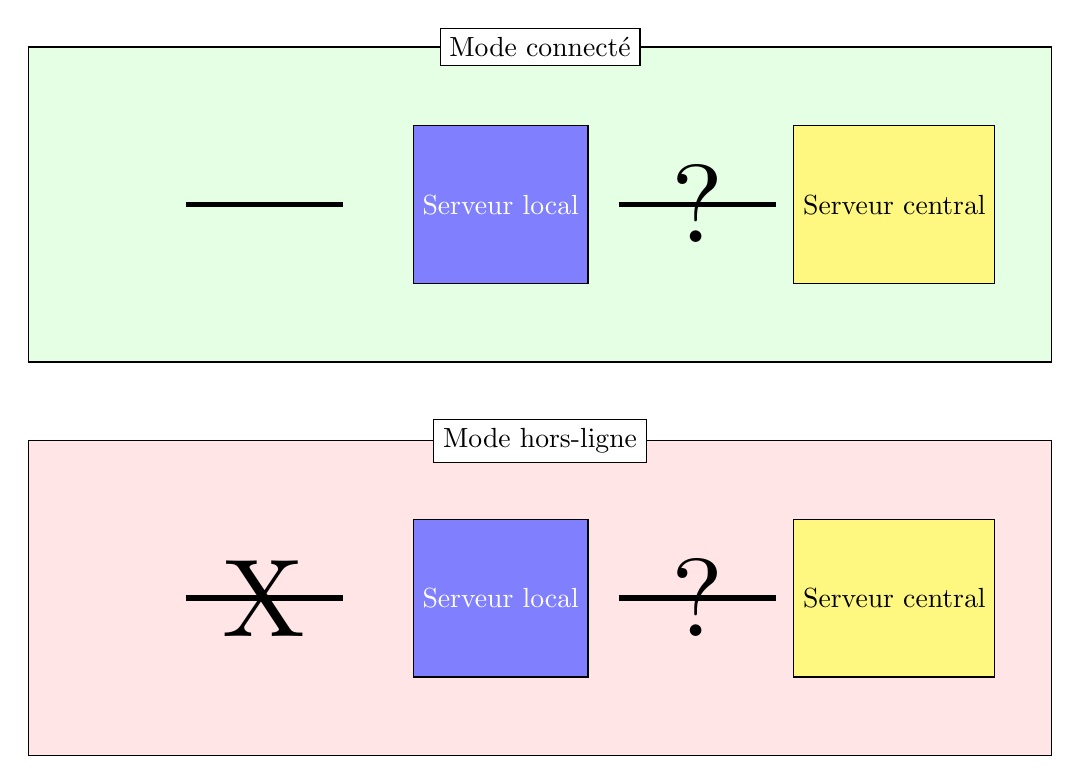
\begin{tikzpicture}
	    % Styles :
		\tikzstyle{titre}=[rectangle,draw,fill=white,text=black]
		\tikzstyle{symbole}=[rectangle,text=black, scale=4]
		\tikzstyle{serveurloc}=[rectangle,draw,fill=blue!50,text=white, minimum height=2cm]
		\tikzstyle{serveurcen}=[rectangle,draw,fill=yellow!50,text=black, minimum height=2cm]
	    % #### CADRE ROUGE :
		% Fond :
		\draw[fill=red!10] (0,0) rectangle (13, 4);
		% Titres :
		\node[titre] at (6.50,4.00) {Mode hors-ligne};
		% Serveurs :
		\node[serveurloc] at (6.00,2) {Serveur local};
		\node[serveurcen] at (11.00,2) {Serveur central};
		\node[symbole] at (8.50,2) {?};
		\node[symbole] at (3.00,2) {X};
		% Traits :
		\draw[line width=2pt] (2, 2) -- (4, 2);
		\draw[line width=2pt] (7.5, 2) -- (9.5, 2);
		% Utilisateurs :
		\umlactor[x=1.00, y=2]{Utilisateur}
		% #### CADRE VERT :
		% Fond :
		\draw[fill=green!10] (0,5) rectangle (13, 9);
		% Titres :
		\node[titre] at (6.50,9.00) {Mode connecté};
		% Serveurs :
		\node[serveurloc] at (6.00,7) {Serveur local};
		\node[serveurcen] at (11.00,7) {Serveur central};
		\node[symbole] at (8.50, 7) {?};
		% Traits :
		\draw[line width=2pt] (2, 7) -- (4, 7);
		\draw[line width=2pt] (7.5, 7) -- (9.5, 7);
		% Utilisateurs :
		\umlactor[x=1.00, y=7]{Utilisateur}
	\end{tikzpicture}
	\caption{Utilisation des modes connecté et hors-ligne}
	\label{explicationcodeco}
\end{figure}
    % TODO Schéma mode connecté
    % TODO Schéma mode hors-ligne
% Fin de la sous-section [Introduction]
% ------------------------------------------------------------------------------

% ------------------------------------------------------------------------------
\subsection{Gestion des priorités \& des profils de synchronisation}
Une priorité permettra à l'application de \og{}choisir\fg{} ce qui transitera sur le réseau. Cinq priorités seront définies (par ordre d'importance croissant) pour qualifier des éléments synchronisables :
\begin{enumerate}
    \item Négligeable
    \item Secondaire
    \item Normal
    \item Important
    \item Crucial
\end{enumerate}
L'utilisateur pourra gérer les priorités à synchroniser en les associant à un profil : lorsque l'utilisateur choisit un profil de synchronisation, seuls les éléments ayant une priorité inclue dans le profil sont synchronisés.
% Diagramme des CU pour la gestion des profils et des priorités :
\begin{figure}[htbp]
    \centering
	\begin{tikzpicture}
		\begin{umlsystem}[x=8.00,y=5.00,fill=yellow!10]{Priorités des éléments synchronisables}
			\umlusecase[x=0.00,y=1.00,name=MPrio]{Modifier la priorité d'un élément}
		\end{umlsystem}
		\begin{umlsystem}[x=8.00,y=0.00,fill=blue!10]{Profils de synchronisation}
			\umlusecase[x=0.00,y=0.00,name=ChProf]{Choisir un profil}
			\umlusecase[x=0.00,y=1.00,name=EProf]{Éditer un profil}
			\umlusecase[x=0.00,y=2.00,name=CrProf]{Creer un profil}
			\umlusecase[x=0.00,y=3.00,name=SProf]{Supprimer un profil}
		\end{umlsystem}
		\umlactor[x=0.00,y=3.00]{Utilisateur}
		\umlassoc{Utilisateur}{MPrio}
		\umlassoc{Utilisateur}{ChProf}
		\umlassoc{Utilisateur}{EProf}
		\umlassoc{Utilisateur}{CrProf}
		\umlassoc{Utilisateur}{SProf}
	\end{tikzpicture}
	\caption{Diagramme des cas d'utilisation pour la synchronisation}
	\label{ucsynchro}
\end{figure}
% Fin de la sous-section [Gestion des priorités]
% ------------------------------------------------------------------------------

% ------------------------------------------------------------------------------
\subsection{Mode connecté}
Dans ce mode, on suppose qu'il y a une liaison réseau entre l'utilisateur et le serveur local; toutes les modifications sont effectuées en \og{}temps réel\footnote{Un écart de temps pourra être constaté dans le cas où le réseau n'offre qu'un faible débit.}\fg{}. Pour ce mode, l'utilisateur doit :
\begin{enumerate}
    \item Se connecter
    \item Utiliser la suite logicielle
    \item Se déconnecter après utilisation
\end{enumerate}
L'utilisateur ne pourra effectuer que les modifications dont il a les \emph{permissions}.
% Diagramme des CU pour le mode connecté :
\begin{figure}[htbp]
    \centering
	\begin{tikzpicture}
		\begin{umlsystem}[x=5.00,y=0.00,fill=green!10]{Mode connecté}
			\umlusecase[x=1.00,y=1.50,name=Co]{Se connecter}
			\umlusecase[x=0.00,y=3.00,name=Modif, width=2cm]{Effectuer des modifications}
			\umlusecase[x=6.00,y=1.50,name=ChMode, width=2cm]{Choisir le mode connecté}
			\umlusecase[x=0.00,y=0.00,name=Deco]{Se déconnecter}
		\end{umlsystem}
		\umlactor[x=1.00,y=1.00]{Utilisateur}
		\umlinclude{Co}{ChMode}
		\umlinclude{Deco}{Co} 
		\umlinclude{Modif}{Co} 
		\umlassoc{Utilisateur}{Co}
		\umlassoc{Utilisateur}{Modif}
		\umlassoc{Utilisateur}{Deco}
	\end{tikzpicture}
	\caption{Diagramme des cas d'utilisation pour le mode connecté}
	\label{ucmodeco}
\end{figure}
% Fin de la sous-section [Mode connecté]
% ------------------------------------------------------------------------------

% ------------------------------------------------------------------------------
\subsection{Mode hors-ligne}
Contrairement au mode conecté, le mode hors ligne permet à l'utilisateur de modifier toutes les informations dont il dospose localement. Lorsqu'il souhaitera synchroniser ses informations avec le serveur, il devra se connecter et c'est à ce moment là que le serveur vérifiera que l'utilisateur n'outrepasse pas les droits qui lui sont accordés. Si c'est le cas, le serveur rejettera les modifications locales.
% Diagramme des CU pour le mode hors ligne :
\begin{figure}[htbp]
    \centering
	\begin{tikzpicture}
		\begin{umlsystem}[x=5.00,y=0.00,fill=red!10]{Mode hors-ligne}
			\umlusecase[x=4.50,y=0.20,name=Co]{Se connecter}
			\umlusecase[x=0.00,y=3.00,name=Modif, width=2cm]{Effectuer des modifications}
			\umlusecase[x=6.00,y=3.00,name=ChMode, width=2cm]{Choisir le mode hors-ligne}
			\umlusecase[x=0.00,y=1.00,name=Sync, width=2cm]{Synchroniser avec le serveur}
		\end{umlsystem}
		\umlactor[x=1.00,y=1.00]{Utilisateur}
		\umlinclude{Co}{ChMode}
		\umlinclude{Sync}{Co} 
		\umlassoc{Utilisateur}{Modif}
		\umlassoc{Utilisateur}{Sync}
	\end{tikzpicture}
	\caption{Diagramme des cas d'utilisation pour le mode hors-ligne}
	\label{ucmodedeco}
\end{figure}
% Fin de la sous-section [Mode hors-ligne]
% ------------------------------------------------------------------------------

% ------------------------------------------------------------------------------
\subsection{Gestion des conflits}
Durant la synchronisation, que ce soit en mode connecté ou hors-ligne, des conflits peuvent survenir au niveau du contenu des informations. Dans ce cas, l'utilisateur est averti du conflit et des informations qu'il touche et il lui revient le soin de les gérer en choisissant explicitement ce qui est correct et qui doit être enregistré sur le serveur.\\
Afin de savoir si la version des informations sur le serveur est plus récente (ou plus vieille) que la version locale, un horodatage est mis en place tel que :
\begin{itemize}
    \item Chaque modification locale est horodatée avec l'heure locale
    \item À la synchronisation, l'écart temporel entre l'heure locale et l'heure serveur est mesuré\footnote{Par exemple, supposons que la machine locale retarde de deux heures : si une information a été modifiée à 17h (heure serveur) et qu'une modification est apportée à 16h le même jour en local, l'écart de deux heures entre les deux machines est mesuré lors de la synchronisation (i.e. deux heures) et permet de dater réellement la modification en local et ainsi déterminer laquelle succède à l'autre. À cette fin, l'application enregistre les éventuels changements d'heure oppérés en local pour notifier le serveur des écarts d'horodatage.}
\end{itemize}
% Fin de la sous-section [Gestin des conflits]
% ------------------------------------------------------------------------------

% Fin de la section [Synchronisation]
% ==============================================================================

